\documentclass{beamer}
%%%%%%%%%%%%%%%%%%%%%%%%%%%%%%%%%%%%%%%%%%%%%%%%%%%%%%%%%%%%%%%%%%%%%%%%%%%%%%%%%%%%%%%%%%%%%%%%%%
\setbeamertemplate{navigation symbols}{}
\usepackage{beamerthemeshadow}
\usefonttheme{serif}
%%%%%%%%%%%%%%%%%%%%%%%%%%%%%%%%%%%%%%%%%%%%%%%%%%%%%%%%%%%%%%%%%%%%%%%%%%%%%%%%%%%%%%%%%%%%%%%%%%
\usepackage{graphicx}
\graphicspath{ {res/} }
%%%%%%%%%%%%%%%%%%%%%%%%%%%%%%%%%%%%%%%%%%%%%%%%%%%%%%%%%%%%%%%%%%%%%%%%%%%%%%%%%%%%%%%%%%%%%%%%%%
\usepackage{polyglossia}
\setdefaultlanguage{armenian}
\setotherlanguages{english}
\usepackage{fontspec}
\newfontfamily\armenianfont{DejaVu Sans}
%%%%%%%%%%%%%%%%%%%%%%%%%%%%%%%%%%%%%%%%%%%%%%%%%%%%%%%%%%%%%%%%%%%%%%%%%%%%%%%%%%%%%%%%%%%%%%%%%%
\usepackage{minted}
\setminted[cpp]{fontsize=\footnotesize}
\setmonofont{Consolas}
%%%%%%%%%%%%%%%%%%%%%%%%%%%%%%%%%%%%%%%%%%%%%%%%%%%%%%%%%%%%%%%%%%%%%%%%%%%%%%%%%%%%%%%%%%%%%%%%%%
\usepackage{xltxtra}
\usepackage{hyperref}
%%%%%%%%%%%%%%%%%%%%%%%%%%%%%%%%%%%%%%%%%%%%%%%%%%%%%%%%%%%%%%%%%%%%%%%%%%%%%%%%%%%%%%%%%%%%%%%%%%
\usetheme{Luebeck}
\usecolortheme{crane}
%%%%%%%%%%%%%%%%%%%%%%%%%%%%%%%%%%%%%%%%%%%%%%%%%%%%%%%%%%%%%%%%%%%%%%%%%%%%%%%%%%%%%%%%%%%%%%%%%%
\definecolor{HTDark}{rgb}{0.04706, 0.13725, 0.26667} % primary color
\definecolor{HTLight}{rgb}{0.3686, 0.5255, 0.6235}   % secondary color
\setbeamercolor{palette primary}{bg=HTDark,fg=white}
\setbeamercolor{palette secondary}{bg=HTDark,fg=white}
\setbeamercolor{palette tertiary}{bg=HTDark,fg=white}
\setbeamercolor{palette quaternary}{bg=HTDark,fg=white}
\setbeamercolor{structure}{fg=HTDark} % itemize, enumerate, etc
\setbeamercolor{section in toc}{fg=HTDark} % TOC sections
\setbeamercolor{block title}{fg=white,bg=HTDark}
\setbeamercolor{block body}{fg=white, bg=HTLight}
\setbeamercolor{subsection in head/foot}{bg=HTLight,fg=white}
%%%%%%%%%%%%%%%%%%%%%%%%%%%%%%%%%%%%%%%%%%%%%%%%%%%%%%%%%%%%%%%%%%%%%%%%%%%%%%%%%%%%%%%%%%%%%%%%%%


\begin{document}

\title[Composite]{Նախագծման Ձևանմուշներ։ Composite}
\author[Հրաչյա Թանդիլյան\copyright]{Հրաչյա Թանդիլյան}
\date{2020}

%-------------------------------------------------------------------------------------------------
\begin{frame}
\titlepage
\end{frame}
%-------------------------------------------------------------------------------------------------

\section{Նպատակը}
%-------------------------------------------------------------------------------------------------
\begin{frame}\frametitle{Composite}
\begin{block}{Նպատակը}
    Խմբավորել օբյեկտները ծառատիպ կառուցվածքներում ամբողջական հիերարխիաներ
    ներկայացնելու համար: \\ Այս Ն.Ձ. թույլ է տալիս միանման դիտարկել և՛ անհատական
    օբյեկտները, և՛ նրանց խմբերը:
\end{block}
\vfill
Նաև հայտնի է որպես
\begin{itemize}
    \item Այլ լայնորեն կիրառվող անուներ չկան:
\end{itemize}
\end{frame}
%-------------------------------------------------------------------------------------------------

\subsection{Մոտիվացիան}
%-------------------------------------------------------------------------------------------------
\begin{frame}\frametitle{Մոտիվացիան}
\begin{center}
    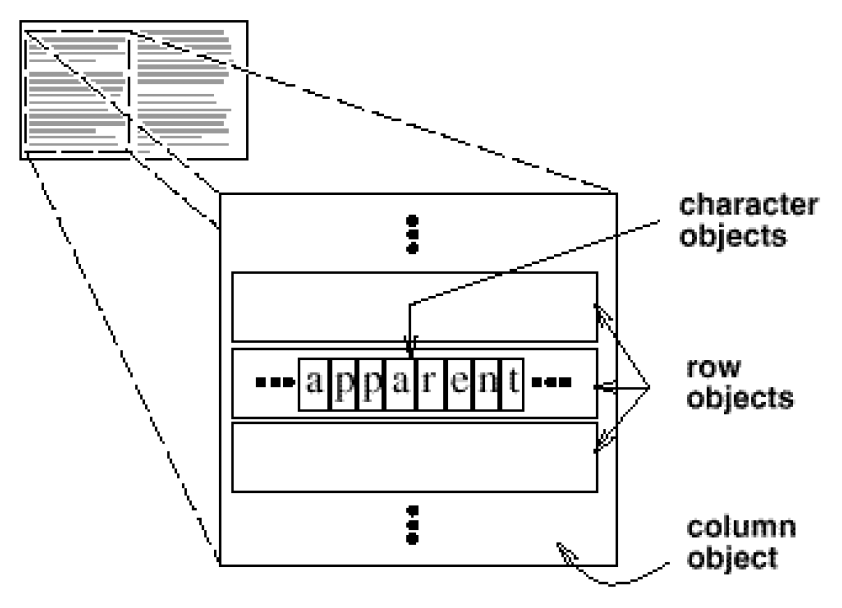
\includegraphics[scale=0.4]{motivation1.png}
\end{center}
\end{frame}
%-------------------------------------------------------------------------------------------------

%-------------------------------------------------------------------------------------------------
\begin{frame}\frametitle{Մոտիվացիան}
\begin{center}
    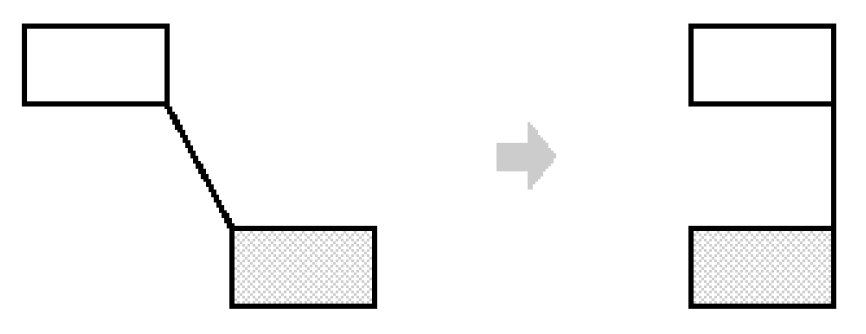
\includegraphics[scale=0.4]{motivation2.png}
\end{center}
\end{frame}
%-------------------------------------------------------------------------------------------------

\subsection{Կիրառելիությունը}
%-------------------------------------------------------------------------------------------------
\begin{frame}\frametitle{Կիրառելիությունը}
Այս Ն.Ձ. պետք է օգտագործել երբ.
\vfill
\begin{enumerate}
    \item Անհրաժեշտ է ներկայացնել օբյեկտների ամբողջական հիերարխիաներ: \pause \vfill
    \item Անհրաժեշտ է, որ օգտագործողը հնարավորություն ունենա թափանցիկ կերպով
    օգտագործել կոմպոզիտ և անհատական օբյեկտները, անտեսել նրանց տարբերությունները:
\end{enumerate}
\end{frame}
%-------------------------------------------------------------------------------------------------

\section{Կառուցվածքը}
%-------------------------------------------------------------------------------------------------
\begin{frame}\frametitle{Կառուցվածքը}
\begin{center}
    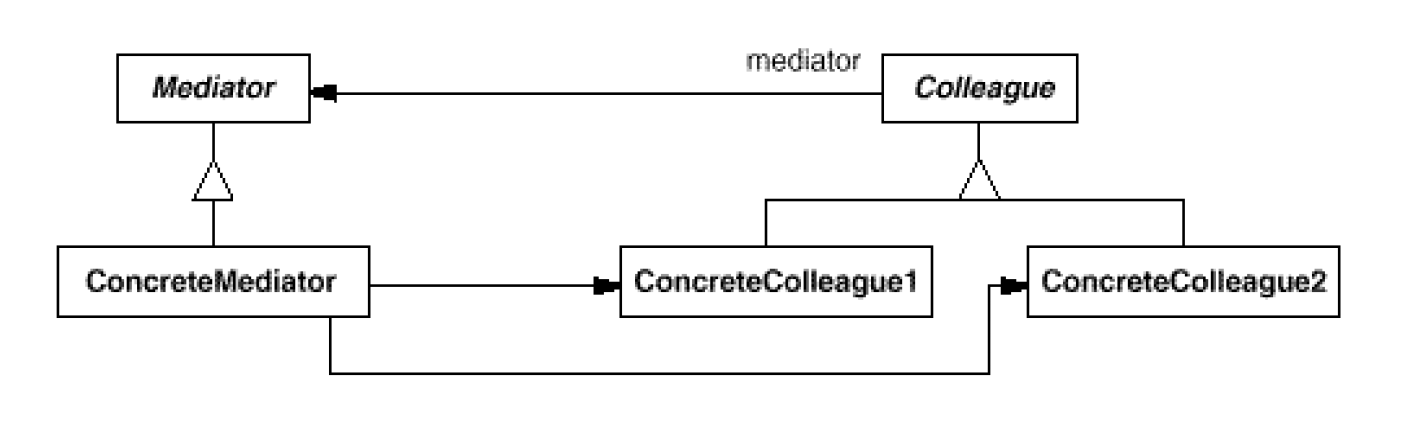
\includegraphics[scale=0.4]{structure1.png}
\end{center}
\end{frame}
%-------------------------------------------------------------------------------------------------

%-------------------------------------------------------------------------------------------------
\begin{frame}\frametitle{Կառուցվածքը}
\begin{center}
    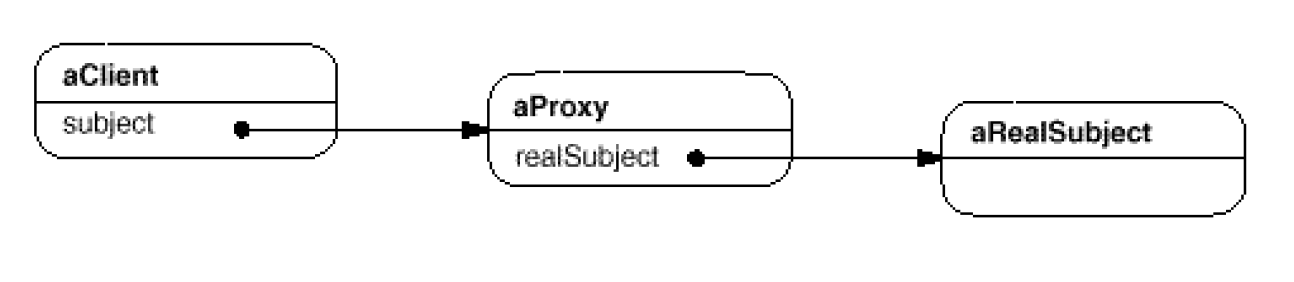
\includegraphics[scale=0.4]{structure2.png}
\end{center}
\end{frame}
%-------------------------------------------------------------------------------------------------

\subsection{Հետևանքները}
%-------------------------------------------------------------------------------------------------
\begin{frame}\frametitle{Հետևանքները}
Այս Ն.Ձ. ունի հետևյալ առավելություններն ու թերությունները.
\vfill
\begin{enumerate}
    \item Սահմանում է օբյեկտների հիերարխիա: \pause \vfill
    \item Պարզեցնում է օգտագործողի կոդը: \pause \vfill
    \item Հեշտացնում է նոր տիպի կոմպոնենտների ավելացումը: \pause \vfill
    \item Նախագծի չափազանց ընդհանրություն:
\end{enumerate}
\end{frame}
%-------------------------------------------------------------------------------------------------

\section{Իրականացումը}
%-------------------------------------------------------------------------------------------------
\begin{frame}\frametitle{Իրականացումը}
\begin{enumerate}
    \item Բացահայտ հղում ծնողին: \vfill
    \item Կոմպոնենտների համատեղ օգտագործում: \vfill
    \item Կոմպոնենտի ինտերֆեյսի մաքսիմիզացում: \vfill
    \item Զավակ կոմպոնենտների ղեկավարման գործողությունների նկարագրում: \vfill
    \item Անհրաժեշտ է արդյոք զավակ կոմպոնենտների ցուցակը սահմանել Component դասում:
\end{enumerate}
\end{frame}
%-------------------------------------------------------------------------------------------------

%-------------------------------------------------------------------------------------------------
\begin{frame}\frametitle{Իրականացումը}
\begin{enumerate}
    \setcounter{enumi}{5}
    \item Զավակների կարգավորումը: \vfill
    \item Քեշավորում արագության բարելավման համար: \vfill
    \item Ով պետք է ջնջի կոմպոնենտները: \vfill
    \item Որն է կոմպոնենտները պահելու համար լավագույն տվյալների կառուցվածքը:
\end{enumerate}
\end{frame}
%-------------------------------------------------------------------------------------------------

\subsection{Օրինակ}
%-------------------------------------------------------------------------------------------------
\begin{frame}[fragile]\frametitle{Օրինակ}
\begin{english}
\begin{minted}[fontsize=\scriptsize]{cpp}
class Equipment {

public:
    virtual ~Equipment();
    const char* Name() { return name; }
    virtual Watt Power();
    virtual Currency NetPrice();

    virtual void Add(Equipment*);
    virtual void Remove(Equipment*);
    virtual Iterator* CreateIterator();

protected:
    Equipment(const char*);

private:
    const char* name;
};
\end{minted}
\end{english}
\end{frame}
%-------------------------------------------------------------------------------------------------

%-------------------------------------------------------------------------------------------------
\begin{frame}[fragile]\frametitle{Օրինակ}
\begin{english}
\begin{minted}{cpp}
class FloppyDisk : public Equipment {

public:
    FloppyDisk(const char*);
    virtual ~FloppyDisk();
    virtual Watt Power();
    virtual Currency NetPrice();
    virtual Currency DiscountPrice();
};
\end{minted}
\end{english}
\end{frame}
%-------------------------------------------------------------------------------------------------

%-------------------------------------------------------------------------------------------------
\begin{frame}[fragile]\frametitle{Օրինակ}
\begin{english}
\begin{minted}[fontsize=\tiny]{cpp}
class CompositeEquipment : public Equipment {

public:
    virtual ~CompositeEquipment();
    virtual Watt Power();

    virtual Currency NetPrice() {
        std::auto_ptr<Iterator> it(CreateIterator());
        Currency total = 0;

        for (it->First(); !it->IsDone(); it->Next()) {
            total += it->CurrentItem()->NetPrice();
        }
        return total;
    }

    virtual void Add(Equipment*);
    virtual void Remove(Equipment*);
    virtual Iterator* CreateIterator();

protected:
    CompositeEquipment(const char*);

private:
    List equipment;
};
\end{minted}
\end{english}
\end{frame}
%-------------------------------------------------------------------------------------------------

%-------------------------------------------------------------------------------------------------
\begin{frame}[fragile]\frametitle{Օրինակ}
\begin{english}
\begin{minted}{cpp}
class Chassis : public CompositeEquipment {

public:
    Chassis(const char*);
    virtual ~Chassis();
    virtual Watt Power();
    virtual Currency NetPrice();
    virtual Currency DiscountPrice();
};
\end{minted}
\end{english}
\end{frame}
%-------------------------------------------------------------------------------------------------

%-------------------------------------------------------------------------------------------------
\begin{frame}[fragile]\frametitle{Օրինակ}
\begin{english}
\begin{minted}{cpp}
Cabinet* cabinet = new Cabinet("PC Cabinet");
Chassis* chassis = new Chassis("PC Chassis");
cabinet->Add(chassis);

Bus* bus = new Bus("MCA Bus");
bus->Add(new Card("16Mbs Token Ring"));
chassis->Add(bus);

chassis->Add(new FloppyDisk("3.5in Floppy"));

cout << "The net price is " << chassis->NetPrice() << endl;
\end{minted}
\end{english}
\end{frame}
%-------------------------------------------------------------------------------------------------

\section{Առնչվող Ձևանմուշները}
%-------------------------------------------------------------------------------------------------
\begin{frame}\frametitle{Առնչվող Նախագծման Ձևանմուշները}
\begin{itemize}
    \item Chain of Responsibility \vfill
    \item Decorator \vfill
    \item Flyweight \vfill
    \item Iterator \vfill
    \item Visitor
\end{itemize}
\end{frame}
%-------------------------------------------------------------------------------------------------

\end{document}
